\section{Progettazione di Dettaglio e Codifica}
\textit{Dal 2021-03-08 al 2021-04-02}

\begin{figure}[H]
	\centering
	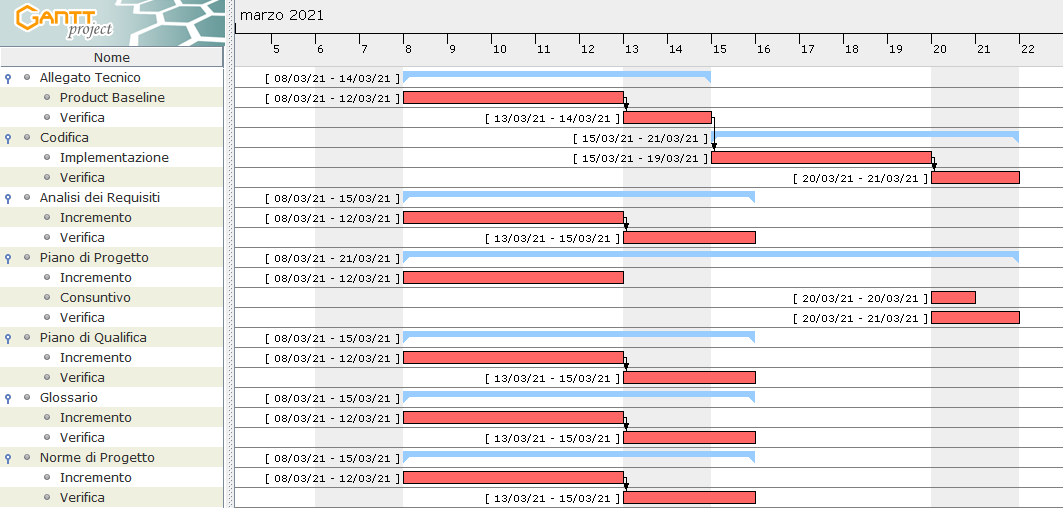
\includegraphics[scale=0.52]{res/images/04_gantt_codifica_obbligatori.png}
	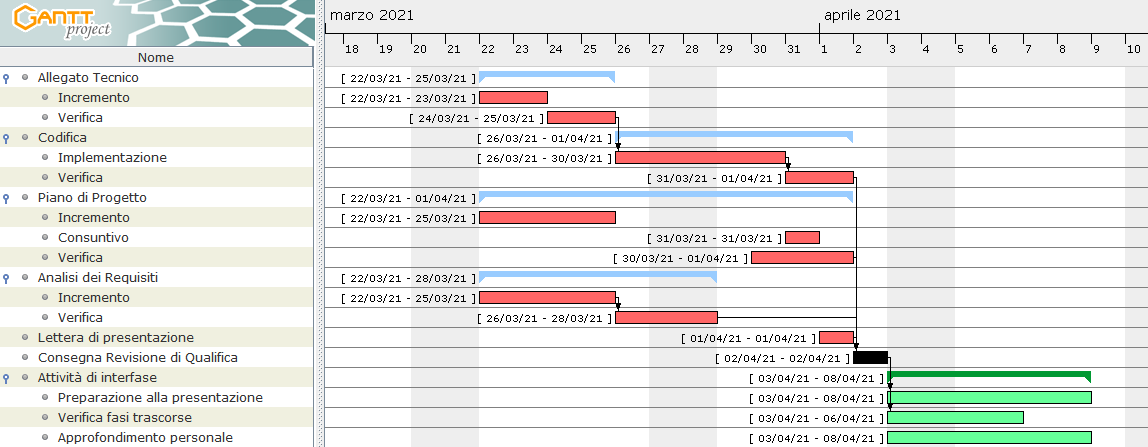
\includegraphics[scale=0.48]{res/images/05_gantt_codifica_desiderabili.png}
	\caption{Diagramma di gantt\textsubscript{G} relativo alla fase\textsubscript{G} di Progettazione  e Codifica}
\end{figure}


\subsection{Periodo 1}

\subsubsection{Pianificazione preventiva}

\paragraph{Attività}

\planningTable{
	Allegato Tecnico & Viene integrato l'\textsc{Allegato Tecnico}, che presenterà ora anche la Product Baseline, nella quale il software è scomposto e analizzato nelle sue unità. & 40 & Progettista
\tabularnewline 
Incremento Analisi dei Requisiti & L'avanzamento nello sviluppo del prodotto chiarirà alcuni aspetti che nella fase\textsubscript{G} di Analisi risultavano oscuri, e potrebbe evidenziare delle criticità non inizialmente considerate. Se necessario, viene raffinata l'\textsc{Analisi dei Requisiti}. & 6 & Analista
\tabularnewline 
Incremento Piano di Progetto & Il \textsc{Piano di Progetto} integrato con il consuntivo del periodo\textsubscript{G} trascorso & 3 & Responsabile
\tabularnewline 
Incremento Glossario & Viene integrato con nuovi termini. & 1 & Responsabile
\tabularnewline 
Incremento Piano di Qualifica & Il cruscotto\textsubscript{G} viene aggiornato con i dati rilevati sul periodo\textsubscript{G} trascorso & 8 & Verificatore
\tabularnewline 
\caption{Pianificazione preventiva - Progettazione di Dettaglio e Codifica - Periodo 1}
}

\paragraph{Preventivo}

\subsubsection{Pianificazione di periodo}

% gantt\textsubscript{G} @nicolò

\paragraph{Attività}



\paragraph{Preventivo orario ed economico}



\subsubsection{Riscontro di fine periodo}


\paragraph{Consuntivo orario ed economico}


\paragraph{Preventivo a finire}





\subsection{Periodo 2}

\subsubsection{Pianificazione preventiva}

\paragraph{Attività}

\planningTable{
	Incremento 1 & Implementazione sistema di autenticazione per i gestori del magazzino. & 20 & Progettista, Programmatore, Verificatore
\tabularnewline 
Incremento 2.A & Aggiunta possibilità di guida manuale dei muletti. & 10 & Progettista, Programmatore, Verificatore
\tabularnewline 
Incremento 2.B & Implementazione di un algoritmo efficiente per la ricerca del miglior percorso per raggiungere la destinazione. & 15 & Progettista, Programmatore, Verificatore
\tabularnewline 
Incremento 2.C & Realizzazione di un algoritmo per la rilevazione e gestione delle collisioni tra le unità. & 20 & Progettista, Programmatore, Verificatore
\tabularnewline 
Incremento 3 & Implentazione dei sensi di percorrenza nella mappa. & 10 & Progettista, Programmatore, Verificatore
\tabularnewline 
Incremento 4.A & Presentazione della mappa del magazzino tramite interfaccia realizzata in Angular.js. & 30 & Progettista, Programmatore, Verificatore
\tabularnewline 
Incremento 4.B & Ideazione e implementazione tool di creazione e modifica della mappa. & 35 & Progettista, Programmatore, Verificatore
\tabularnewline 
Incremento 4.C & Realizzazione pannello di guida dell'unità nell'interfaccia grafica, e finestra di visualizzazione delle task delle unità. & 20 & Progettista, Programmatore, Verificatore
\tabularnewline 
Incremento 4.D & Realizzazione pannello di visualizzazione delle task da svolgere e completate. & 10 & Progettista, Programmatore, Verificatore
\tabularnewline 
Incremento 5.A & Collegamento tra server, frontend e unità. & 20 & Progettista, Programmatore, Verificatore
\tabularnewline 
Incremento 5.B & Studio e applicazione di Containter Docker alle componenti del sistema. & 20 & Progettista, Programmatore, Verificatore
\tabularnewline 
Incremento 6 (opzionale) & Implementazione della velocità modulabile delle unità. & 15 & Progettista, Programmatore, Verificatore
\tabularnewline 
Incremento 7 (opzionale) & Aggiunta e implementazione di attore "pedone". & 30 & Progettista, Programmatore, Verificatore
\tabularnewline 
\caption{Pianificazione preventiva - Progettazione di Dettaglio e Codifica - Periodo 2}
}

\paragraph{Preventivo}

\subsubsection{Pianificazione di periodo}


% gantt\textsubscript{G} @nicolò


\paragraph{Attività}

\paragraph{Preventivo orario ed economico}



\subsubsection{Riscontro di fine periodo}


\paragraph{Consuntivo orario ed economico}


\paragraph{Preventivo a finire}






\subsection{Periodo 3}

\subsubsection{Pianificazione preventiva}

\paragraph{Attività}

\planningTable{
	Preparazione alla presentazione & Viene preparato il materiale necessario alla presentazione. & 7 & Amministratore
\tabularnewline 
Verifica dei macro periodi precedenti & Il gruppo si vede coinvolto in un confronto dal quale vorranno emergere le criticità riscontrate nel macro periodo\textsubscript{G} trascorso, al fine di migliorare lo svolgimento dei periodi successivi. & 1 & Responsabile
\tabularnewline 
Approfondimento personale & Ogni membro del gruppo spende alcune ore per formare e consolidare una conoscenza di base degli strumenti e tecniche da impiegare nel periodo\textsubscript{G} successivo. & 4 & Progettista
\tabularnewline 
\caption{Pianificazione preventiva - Progettazione di Dettaglio e Codifica - Periodo 3}
}

\paragraph{Preventivo}

\subsubsection{Pianificazione di periodo}


% gantt\textsubscript{G} @nicolò


\paragraph{Attività}


\paragraph{Preventivo orario ed economico}



\subsubsection{Riscontro di fine periodo}


\paragraph{Consuntivo orario ed economico}


\paragraph{Preventivo a finire}
